\documentclass[11pt]{article}
\usepackage[T1]{fontenc}
\usepackage[francais]{babel}
\usepackage{array}
\usepackage{shortvrb}
\usepackage{listings}
\usepackage[fleqn]{amsmath}
\usepackage{amsfonts}
\usepackage{fullpage}
\usepackage{enumerate}
\usepackage{graphicx}             % import, scale, and rotate graphics
\usepackage{subfigure}            % group figures
\usepackage{alltt}
\usepackage{url}
\usepackage{indentfirst}
\usepackage{eurosym}
\usepackage{amsmath} 
\usepackage{float}
\usepackage[french,onelanguage,ruled,vlined]{algorithm2e}
%\usepackage{algorithm, algpseudocode}
%\usepackage{tabular}
\usepackage[utf8]{inputenc}
\usepackage{algpseudocode}

%Définition du c pour les "listings"
\usepackage{listings}
\usepackage{xcolor}
\definecolor{mGreen}{rgb}{0,0.6,0}
\definecolor{mGray}{rgb}{0.5,0.5,0.5}
\definecolor{mPurple}{rgb}{0.58,0,0.82}
\definecolor{backgroundColour}{rgb}{0.95,0.95,0.92}

\lstdefinestyle{CStyle}{
    backgroundcolor=\color{backgroundColour},   
    commentstyle=\color{mGreen},
    keywordstyle=\color{magenta},
    numberstyle=\tiny\color{mGray},
    stringstyle=\color{mPurple},
    basicstyle=\footnotesize,
    breakatwhitespace=false,         
    breaklines=true,                 
    captionpos=b,                    
    keepspaces=true,                 
    numbers=left,                    
    numbersep=5pt,                  
    showspaces=false,                
    showstringspaces=false,
    showtabs=false,                  
    tabsize=2,
    language=C
}


\begin{document}
\begin{titlepage}

   \begin{figure}[htbp]
      \centering
      
\includegraphics{img/uliege-logo-couleurs-300.jpg}
   \end{figure}
  	
  	\hfill

	\begin{center}
		\vfill
		\textbf{
		\Huge{MATH0499-1 Théorie des Graphes}}\\
		\bigskip
		\huge{Enumération de circuits et chemins hamiltoniens \\Le parcours du cavalier}\\
		\bigskip %saut de ligne
		\smallskip
		\Large{Mazurchyk Aliaksei\\Antoine Sadzot} \\
		\bigskip
		\smallskip
		\large{\today}\\%date
		\vfill
		\large{Université de Liège}
	\end{center}
\end{titlepage}
	%Presentation du projet

\clearpage
\tableofcontents
\clearpage

\section{Présentation du projet}

\subsection{Énoncé}
Lorsque nous avons sélectionné notre projet, l'énoncé d'origine était le suivant : \\
\enquote{Étant donné un échiquier de dimension $m \times n$, énumérer tous les circuits hamiltoniens réalisés en utilisant uniquement les mouvements du cavalier dans le jeu d'échecs. Même question, mais en énumérant le nombre de chemins hamiltoniens "ouverts" (origine et destination différentes).}

A cet énoncé, nous avons décidé d'ajouter une autre partie : \\
\enquote{Étant donné un échiquier de dimension $m \times n$, générer et afficher un circuit (ou un chemin) hamiltonien basé uniquement sur les mouvements du cavalier.}
\subsection{Les bases du problème du cavalier}
Le problème du cavalier peut donc être représenté sous la forme d'un graphe. Chaque case de l'échiquier est un sommet et chaque mouvement possible à partir de cette case vers une autre case est une arête du graphe.

\begin{figure}[h]
\begin{center}
   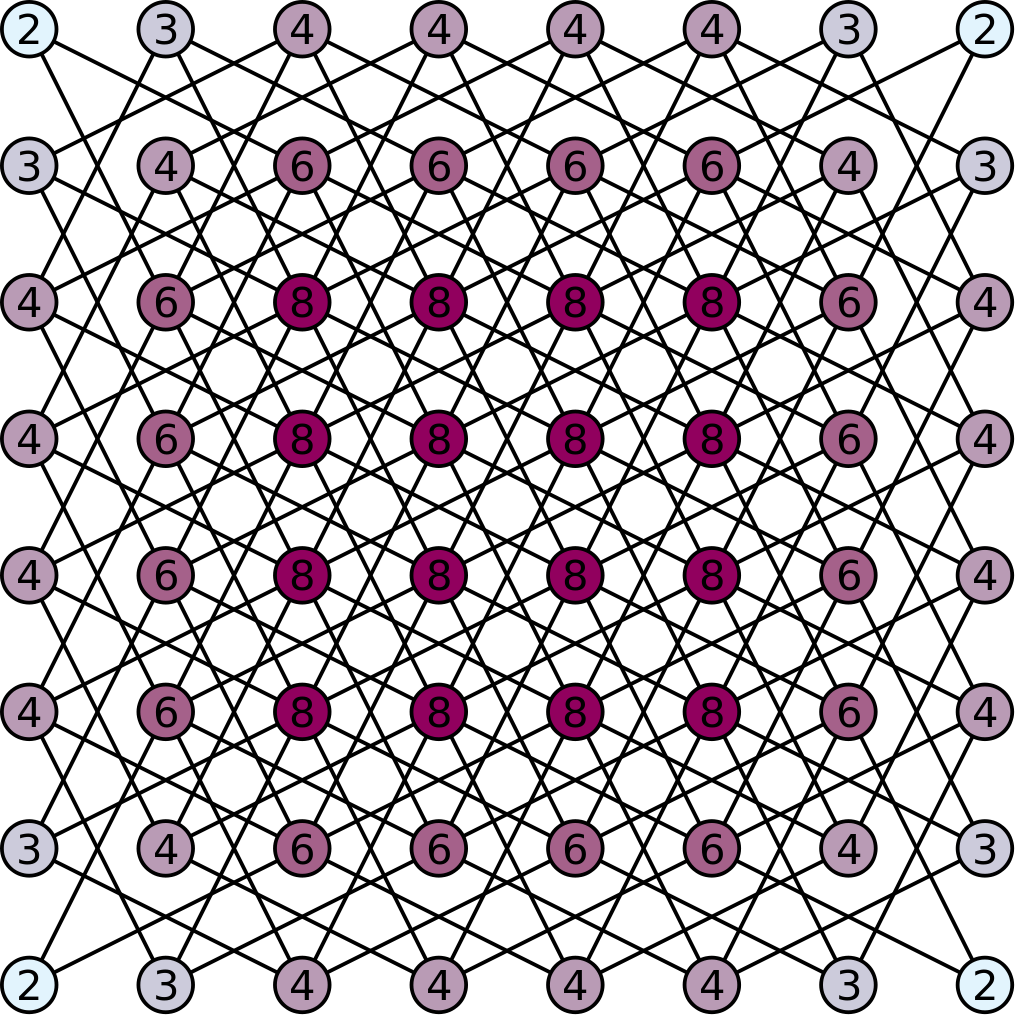
\includegraphics[scale=0.25]{img/graph_cavalier.png} 
   \caption{\label{cavalier_graphe} Graphe du cavalier sur un échiquier $8 \times 8$(inclure source ici wiki)}
   \end{center}
\end{figure}

Le graphe de la figure ~\ref{cavalier_graphe} représente les déplacements possibles pour un cavalier sur un échiquier classique. Le chiffre attribué à chaque case représente le nombre de cases accessibles en un mouvement depuis celle-ci. La réalisation de ce travail implique la génération d'un graphe similaire, généralisé à n'importe quelle taille $m \times n$. 

Le graphe ainsi généré peut ensuite être exploité pour y trouver des chemins et circuits hamiltoniens.

	%Presentation du projet
\section{Recherches}
\subsection{Condition d'existence}
Allen J. Schwenk démontra en 1991 que trois conditions empêchent la réalisation d'un tour de cavalier sur un échiquier rectangulaire $m \times n$  pour tout $m \leq n$. Si aucune de ces condition n'est remplie alors au moins un circuit hamiltonien existe (par extension un chemin hamiltonien existe également).
\begin{enumerate}
\item $m$ et $n$ sont impaires
\item $m = 1,2,$ ou $4$
\item $m = 3$ et $n = 4,6$ ou $8$
\end{enumerate}

\subsection{Algorithmes de parcourt}
Le problème du cavalier étant connu et étudié depuis plusieurs siècles, un certain nombre d'algorithmes existent pour trouver un circuit ou un chemin hamiltonien.

\subsubsection{Force brute}
\subsubsection{Warnsdorf}
La "Loi de Warnsdorff" est une heuristique développée par H. C. von Warnsdorff en 1823 qui permet de trouver un chemin hamiltonien sur un échiquier carré. L'heuristique se base sur le graphe présenté en figure ~\ref{cavalier_graphe} où chaque nœud se voit attribuer un poids correspondant au nombre de nœuds accessibles. On démarre le chemin sur un nœud au hasard. De ce nœud, on se déplace vers le nœud de poids le plus faible. Si plusieurs nœuds de même poids sont accessibles, ceux-ci doivent être départagés. La méthode a l'avantage d'avoir une complexité linéaire en aire (n*n). 

La méthode de départage la plus simple est la sélection aléatoire du nœud suivant. Cette méthode peut paraître simpliste, mais elle est redoutablement efficace jusqu'à une certaine taille d'échiquier. L'algorithme a été mis en place dans notre programme et un benchmark est proposé plus loin dans le rapport.

De nombreux mathématiciens se sont basés sur la loi de Warnsdorff pour y incorporer leur propre méthode de départage. Nous nous sommes plus particulièrement intéressés aux travaux de D. Squirrel, qui a élaboré en 1996 une méthode pour départager les candidats. Celle-ci permet de trouver à coup sûr un chemin hamiltonien pour toute taille d'échiquier carré, si tant est que celui-ci existe. Pour ce faire, toutes les cases accessibles depuis une case sont numérotées de 1 à 8 dans le sens horlogique, la 1 étant en haut à gauche et la 8 en haut à droite. Selon la taille de l'échiquier et la position du cavalier, un ordre de parcours est définit. Par exemple : 34261578. Le chiffre à gauche est la première case à visiter et celle à droite est la dernière. Lorsque plusieurs cases ont le même poids, elles sont départagées par cet ordre de parcours. Nous avons retranscrit l'algorithme proposé par Squirrel dans un programme en C. Nous avons pu observer la fiabilité de ses résultats. Sa méthode a également une complexité O(n*n).
\subsubsection{Echiquier rectangulaire}
La forme de l'échiquier influence évidemment les méthodes de recherches du problème du cavalier. Il est à noter que la loi de Warnsdorff avec départage aléatoire peut fonctionner sur des échiquiers rectangulaires, tel que nous l'avons testé. Néanmoins, l'heuristique présente évidemment les mêmes faiblesses que pour les échiquiers carrés.

Nous somme attardés sur les recherches de Shun-Shii Lin et Chung-Liang Wei, qui ont réussi à créer un algorithme pour trouver à coup sur un chemin ou un circuit Hamiltonien sur un échiquier rectangulaire de taille m*n.  A condition qu'un tel chemin existe. Ils se sont basés sur les recherches de Parberry, qui a développé un algorithme basé sur le principe du "diviser pour régner". Avec ce principe, l'échiquier est diviser en petits échiquiers. Un chemin hamiltonien est trouvé pour chaque petit échiquier. Ensuite, les chemins sont reliés ensemble pour former un seul grand échiquier. Par manque de temps, nous n'avons implémenté qu'une partie de l'algorithme, permettant de résoudre le problème avec un échiquier de taille 3*m. Encore une fois avec une complexité O(n*m).

\subsubsection{Réseaux neuronaux}	%Recherches
\section{Implémentation}
\subsection{BruteForce}
L'implémentation de l’algorithme d’énumération de chemins et circuits par force brute utilise la librairie de gestions de graphes mise à disposition des étudiants sur le site discmath. Toute interaction de l’application se fait en ligne de commande via les arguments de l’exécutable. L’utilisateur peut ainsi choisir le type de parcourt ouvert ou fermé ainsi que la taille de l’échiquier en X et en Y.  Cela permet la création de scripts pour automatiser l’exécution qui peut prendre un temps considérable pour des tailles importantes d’échiquier.
Lors de l’initialisation, un graphe représentant les cases accessibles à partir de chaque case est crée. Ensuite une fonction récursive parcourt ce graphe en fonction de la liste d’adjacence de chaque nœud et des cases déjà visitées.

Cet algorithme de parcourt récursif est appelé pour chaque case de départ possible. Cela permet de créer un tableau montrant le nombre de chemins existants en fonction de la position de départ. L’utilisateur peut voir l’évolution du calcul en temps réel dans le terminal.
\begin{table}[H]
\centering
\caption{Tableau crée pour une recherche de chemins sur un échiquier de taille 5*5}
\label{my-label}
\begin{tabular}{lllll}
304 & 0  & 56 & 0  & 304 \\
0   & 56 & 0  & 56 & 0   \\
56  & 0  & 64 & 0  & 56  \\
0   & 56 & 0  & 56 & 0   \\
304 & 0  & 56 & 0  & 304
\end{tabular}
\end{table}
\subsection{Génération de chemins et circuits hamiltoniens}
Pour la partie du code concernant la génération de circuits et chemins sur des échiquiers de taille variable, nous avons implémenté trois fonctions, pour les trois algorithmes sélectionnés :
\begin{itemize}
\item Heuristique de Warnsdorff pour trouver un chemin ou un circuit sur un échiquier carré ou rectangulaire avec départage aléatoire.
\item Algorithme de Squirrel pour trouver à coup sur un chemin sur un échiquier carré.
\item Algorithme de Shun-Shii pour le cas d'un échiquier de trois lignes et m colonnes. Permettant de trouver un chemin hamiltonien.
\end{itemize}
\subsubsection{Génération de parcours et chemins}
Dans ces fonctions, nous enregistrons l'ordre de parcours des cases dans un vecteur A. Le premier élément de ce vecteur représente la case en haut à gauche. Le dernier élément représente la case en bas à droite. Comme si les rangées de l'échiquier avaient été mises bout à bout. Les éléments contiennent comme valeur l'ordre de passage du cavalier sur la case correspondante. Allant donc de 0 à n*m-1. Un vecteur B contient le poids des cases, comme sur la figure ~\ref{cavalier_graphe}. Il est à noter que tous nos algorithmes commencent dans la case en haut à droite de l'échiquier. Théoriquement, l'algorithme avec départage aléatoire pourrait commencer sur n'importe quelle case. Mais par facilité, nous avons décidé arbitrairement de celle-ci.

Afin de minimiser les temps de calcul, le lancement de la fonction de parcourt se fait en multithreading via OpenMP. Ainsi un thread travaille sur chaque case initiale possible.

Au début, nous avions décidé d'utiliser l'interface de génération de graphes vue au cours, en la modifiant légèrement. Cependant, le résultat obtenu avec l'algorithme de Warnsdorff était trop compliqué et trop lent. Nous avons donc décidé de nous inspirer de l'algorithme de Squirrel, basé sur les matrices décrite au paragraphe précédent.
Le fonctionnement des algorithme a été décrit au chapitre précédent. 

\subsubsection{Test de la validité des parcours et chemins}
Pour vérifier la justesse des parcours et chemins générés, nous avons écrit deux fonctions de test. L'une pour les parcours et l'autre pour les chemins. Leur fonctionnement est pratiquement identique. L'algorithme commence à la case "0". On regarde ensuite si la case "1" est accessible en un mouvement de cavalier. Si oui, on s'y déplace,... Si toutes les cases ont pu être visitées, le chemin est valide. Pour le test de circuits, on vérifie en plus si la case "0" est accessible depuis la case "n*n-1".

\subsubsection{Affichage du résultat}
En plus de la génération, nous proposons d'enregistrer le résultat obtenu dans un fichier texte. La figure ~\ref{ExempleImpression} montre plusieurs exemples de parcours générés.

\begin{figure}[h]
\begin{center}
   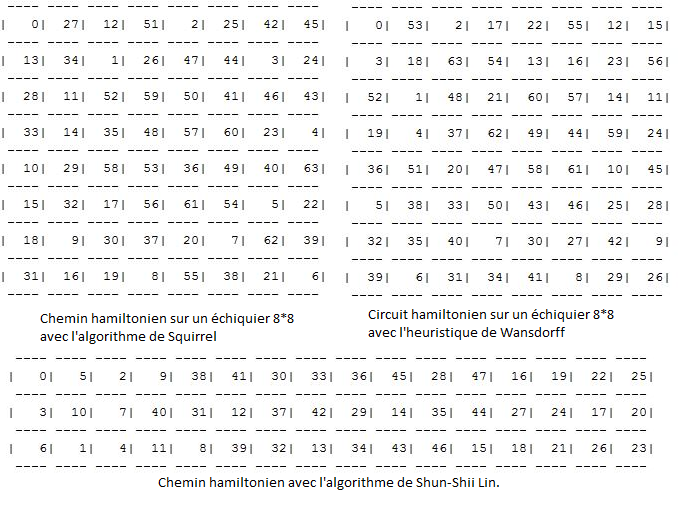
\includegraphics[scale=0.6]{img/exempleimpression.png} 
   \caption{\label{ExempleImpression} Exemple de chemins et circuits générés}
   \end{center}
\end{figure}	%Implémentation
\section{Conclusion}
	%Tests de performance
\section{Conclusion}
	%Conclsion


	
\end{document}
